\chapter{Background}

\large  The internet and computers have played significant role in a transformation of documents. Before documents got digitized, it used to be in form of printed papers. Most of the documents have their own layouts which is highly dependent on the language since the language comes with its own grammatical rules and the way of sentence formation. Once the smartphone came into the world, it started influencing the way of documents being prepared. To understand the text document has always been a part of interest in computer science. Since the impact of having a system that can understand the text document correctly, its repeatable functionality and speed that could help industries or companies to bring down the cost and time they are spending on dealing with documents on their day to day life. However, there are many steps in between to address before machine can read and understand text and layout information in text documents. Start with the letters, words and sentences. These are the basic and prime components of any language. One can not pass any information without it. One can argue about passing information in terms of symbol or a figure but at the basic level a letter is like a symbol or a figure that represents some value or information. We as a human being can easily recognise the texture and the layout of the letter by just looking at it, which is not the case for computers. Till the date computers are using 1s and 0s to perform tasks. Therefore it is a challenge to be able to recognise and process the letters that have been used in word or sentence while generating the document and form a structure of 1s and 0s so that machine can understand. 

\section{Compilers}
The roots of compilers are in 19s, Corrado Böhm wrote first ever practical compiler \cite{Theroy_compiler}. Grace Murray Hopper wrote the first implemented compiler. She also was a part of the team who developed the "UNIVAC \RomanNumeralCaps{1}", the first commercial computer produced  in United States \cite{Grace_Murray_Hopper_History}. Later on she created the first English-Based data processing language FLOW-MATIC, a principal precursor for COBOL - a prime programming language for business applications. Since then, many more compilers introduced with various programming languages. In simple words, Compilers are translator for computers. Through compilers, machines can understand the High-level programming languages like C++, Java, Python and so on. High-level programming languages refer as a language that human can read and write, However it is not possible to execute these lines of High-level programming languages directly by computer's CPU. Therefore the concept of compilers has been introduced in order to translate these high-level programming languages("Source Code") to machine codes, also known as "binary code (1's and 0's)". Compilers takes the Source Code as it is in High-level programming language and breaks it into small chunks (Lexemes). These Lexemes are later on converted to "tokens" for processing. Once the token generation is been done, Using Syntax Analysis and Semantic Analysis, Compilers can check whether if the sequence of tokens meets the requirements of rules and complex issues like function arguments and type compatibility in syntax tree accordingly. Once it is ready, the translation task is being performed in which compilers will generate intermediate code, optimize the code(optional), and generate the machine code.  


\subsubsection{Overview of compiler's functionality}
\begin{listing}[!hb]

        \begin{minted}{C++}
            int main(){
                int a = 5;
                int b = 10;
                return a + b;
            }
        \end{minted}
    
    \caption{Example of Compiler's steps}
    \label{Listing:1}   
\end{listing}


The source code in \Cref{Listing:1} is written in High-level programming language "C++". Compiler will take this code and perform a lexical analysis and generates tokens, that will be represented as int, main, (, ), \{, int a = 5;, int b = 10;, return a + b; and \}. After generating tokens it performs syntax analysis in which it checks whether if these tokens makes sense in order they are in, e.g., we have defined the function \textbf{main} with no arguments and returns \textbf{int}. We have defined two integers \textbf{a} and \textbf{b}, than the function will return the sum of these integers. In the step Symantic Analysis, Compilers checks whether if we are using variables before they're defined? Are we trying to add things like strings that are not integers or numbers? and so on. Finally, the compilers will generate the machine code (1s and 0s) that is specific to the architecture to the machine where it's meant to run on.

\section{Optical Character Recognition (OCR)}
Compilers are specifically design to understand these high-level programming languages and translate it to the machine code, but when it comes to read a document, it is difficult for them since document does not contains the rules similar to programming languages and in addition, every text documents have the basic blocks of any human language "letters". Character recognition techniques refers to a symbolic identity of a character within symbol or a character. This includes the replication/recognition of human functions like machine printed and hand printed/cursive-written characters by machines. Character recognition is known as optical character recognition since it deals with optically processed characters. The first mention of OCR was for as an aid to the visually handicapped and the first successful attempt was achieved by Russian Scientist Tyurin in 1900 \cite{govindan1990character}. Later on, the application of OCR changed into data processing systems in business world since it can deal with the enormous flood of paper documents such as bank cheques, commercial forms, credit card imprints, governmental records, mails and so on. Before smartphones and digital camera, documents were simply printed papers, However since smartphones and digital cameras got introduced, the number of documents increased since documents can now be easily produced digitally. Though generating documents got digitized, not all the documents are in machine readable or processable format. Most of them are just images or scans. Where OCR allowed to deal with these digitally born document such as scanned paper-documents, PDF files or images captured by a digital camera into machine readable, editable and searchable data. In paper \citep{AnOverviewoftheTesseractOCREngine} author have described in detail functionality of methods of famous Tesseract OCR Engine. Author talk about the development of open-source OCR engine "Tesseract" that it was develooped at HP between 1984 and 1994. In the infancy era for Tesseract, the accuracy was a challange, and it was major PhD reserch project in HP Labs Bristol. It was 1994, HP presented the final developed OCR engine to UNLV for the 1995 Annual Test of OCR Accuracy\cite{UNLV_4th_annual_test_ocr}, where it got prooved that it was worth against the commercial engines that exists that time. Later in 2005, HP made Tesseract for open source which is available at \url{http://code.google.com/p/tesseract-ocr}. According to \cite{AnOverviewoftheTesseractOCREngine}, the functionality of Tesseract OCR has been described in upcoming paragraphs.

\subsection{Line and Word Finding}
\subsubsection{Line Finding}

The line finding algorithm was developed to be able to work with images that are skewed without performing de-skew in order to maintain  the image quality \cite{Line_Finding_Algorithem}. The key role of this algorithm is to perform blob filtering and line construction. It uses a \textbf{simple percentile hight filter} for removing drop-caps and vertically touching characters, The \textbf{median height approximation} for text size and region and makes it safe to filter out blobs smaller than some fraction of the median height. By sorting x-coordinates, blobs are assigned to a unique text-lines. Later on, a least median of squares fir \cite{least_median_squares_algorithm} is being used for baseline estimation. Finally all blobs are being merged to form a line.

\subsubsection{Baseline Fitting}

After the line of the text document has been extracted, the baseline are fitted with more accuratly using a quadratic spline, an another first approch for OCR system that allowed Tesseract to handle curved baselines \cite{quadratic_spline_algorithm}. While quadratic spline have an advantage of claculating reasonably stable baseline, it can struggle when it comes to multiple spline segments. Therefore, the more traditional cubic spline \cite{Traditional_cubic_algorithm} has been used to perfom baseline fitting.

\begin{figure}[h]
    \centering
    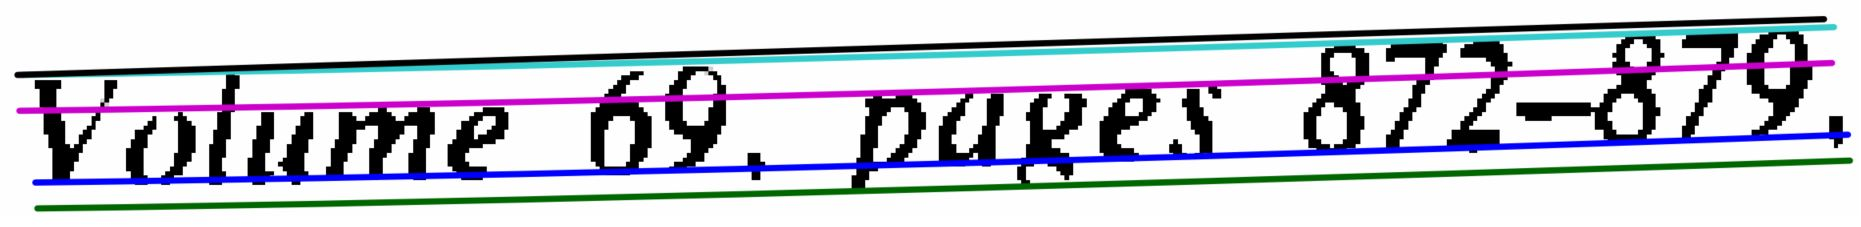
\includegraphics[width=0.7\textwidth]{chapters/images/OCR/Base_Line_Fitting.JPG}
    \caption{An example of a curved fitted baseline \cite{AnOverviewoftheTesseractOCREngine}}
    \label{fig:Baseline_Fitting}
\end{figure}

\Cref{fig:Baseline_Fitting} shows the fitted baseline, descender line, mean-line and ascender line. The black line is straight and cyan line is slightly curved with compare to the straight black line above it.

\subsubsection{Fixed Pitch Detection and Chopping}

Tesseract takes the text lines and finds the fixed pitch and chops the words into characters using the pitch. It also disables the chopper and associator on these words for word recognition. A typical example of chopping fixed-pitch word has been showed in \Cref{fig:Fixed_Pitch_detection}.

\begin{figure}[ht]
    \centering
    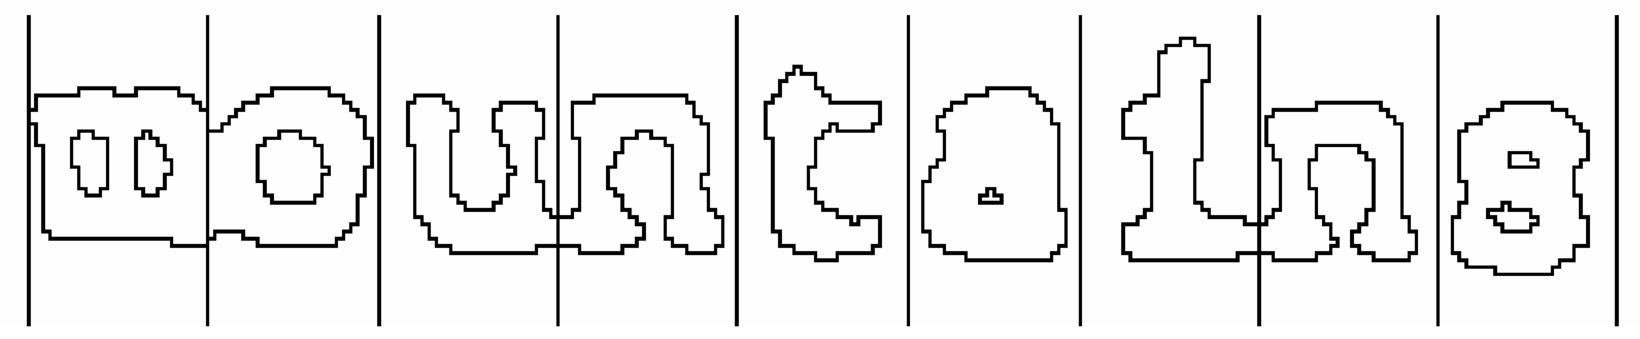
\includegraphics[width=0.7\textwidth]{chapters/images/OCR/Fixed_Pitch_detection.JPG}
    \caption{Fixed Pitch Detection and Chopping\cite{AnOverviewoftheTesseractOCREngine}}
    \label{fig:Fixed_Pitch_detection}
\end{figure}

\subsubsection{Proportional Word Finding}

\Cref{fig:Proportional_Word_Finding} shows a typical exmple of the problems when it comes to perform various task mention in previous paragraphs. For instance, (\RomanNumeralLows{1}) The units of '11.9\%' is clearly larger than the kerned of words 'erated'. (\RomanNumeralLows{2}) There is no horizontal gap at all between words 'of' and 'financial'.

\begin{figure}[ht]
    \centering
    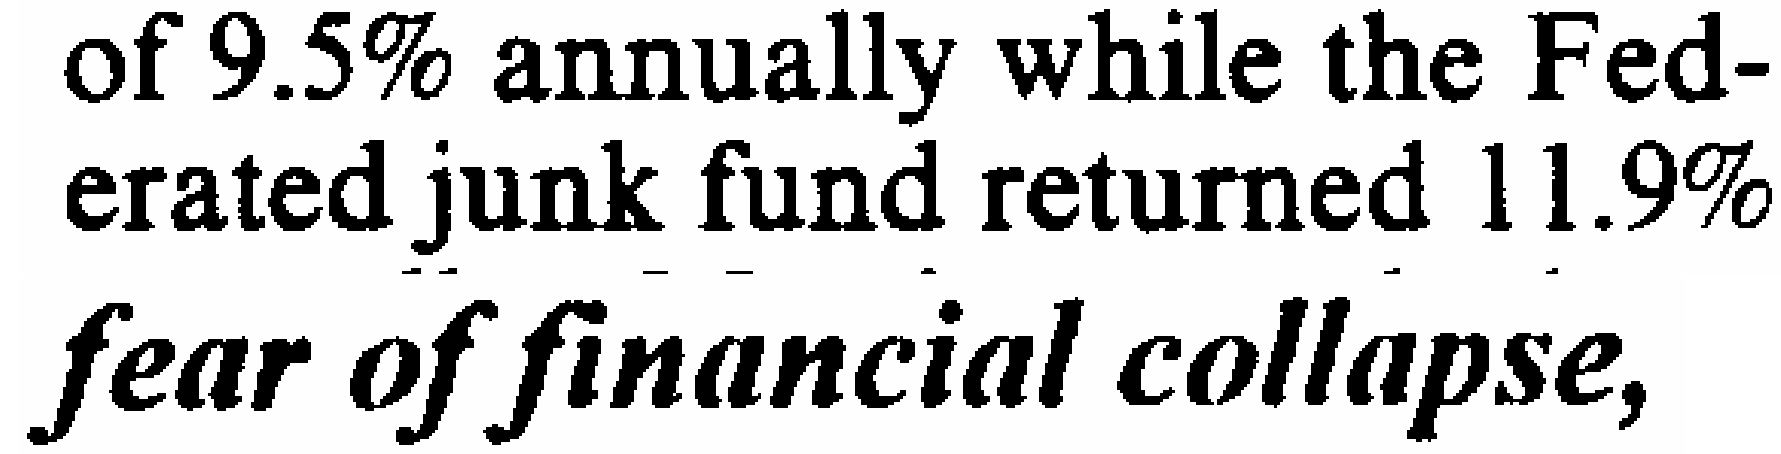
\includegraphics[width=0.6\textwidth]{chapters/images/OCR/Word_Finding.JPG}
    \caption{Proportional Word Finding\cite{AnOverviewoftheTesseractOCREngine}}
    \label{fig:Proportional_Word_Finding}
\end{figure}

Tesseract uses measurements of gaps in limited vertical range between the baseline and mean line. The spaces with smallest threshold are made fuzzy which later will be classified in word recognition.



\subsection{Overview of post process after Line and Word Finding}

Once the lines and words from the documents have been found, the step "Word Recognition" \cite{AnOverviewoftheTesseractOCREngine} is performed to identify the word segmentation which will be letter on classified. Tesseract performs "Chopping Joined Characters" in order to improve the results by chopping the blob based on the confidence derived from classifier. After the elimination of non potential chops, if the word is still not good enough, an associator makes an A* (best first) search based on  segmentation graph of possible combinations. This step can help Tesseract to identify the broken characters with more accuracy. Later on a "Static Character Classifier" \cite{AnOverviewoftheTesseractOCREngine} generates the 3-dimensional, (x, y, position, angle) with 50-100 features and the prototype features are 4-dimensional (x, y, position, angle, length) in a character. Which than will be used to perform classification to assign classes. The results of the Tesseract OCR is then exported to text, word or HTML format.

\section{Machine Translation}

OCR provides ability to extract the letters out of documents and compilers can translate the specific language structure in a way that machine can understand, However, there is some mechanism missing between compiling High-language programming language and understanding the letters, words or sentences derived from parsing the document. Language plays a dominant role in terms of passing information, thoughts and ideas. In addition, different regions, countries and part of the world have different languages that varies in structure, grammar, letters and so on making it difficult to come with the logic or mathematical rule which can apply on one or more languages in order to understand for machines. The early approach of Noam Chomsky \cite{robert1957review}, who introduced syntactic structures as a formalized theory of linguistic structure. He introduced rules based on universal grammar, However languages are generally not well-defined and lack in stable structure hence the approach had several drawbacks. Although, the approach was not perfect, it started the true evolution of NLP. Later on the trend shifted to using probabilities and statistics for machine translation but the progress of slower than expected resulting in less funding. It was the year 1969, Roger Schank presented the concept of using tokens \cite{tokenization_history} which is still being used in NLP, Tokens provided better grasp to map sentences, it can provide better insights to machine with detailed information at object-level. 

In the 1980's, an emerging field of computer science, Machine Learning was progressing significantly in the domain of computing. Algorithms like decision trees provide enough confidence for machine to take decision using if-then rules provided acceptable evidence and new ways to conceptualise the language rather then using handwritten rules. Currently, the trend has been changed to neural networks or deep-learning. Deep-learning became the most efficient way to deal with natural languages since it is not necessary for a programmer to provide rules to decide, algorithm improves the accuracy or efficiency by mapping an input to an output and reducing the errors. 

\section{Transformers}

Self-attention has been used in tasks such as reading comprehension, abstractive summarization, textual entailment and learning task-independent sentence representations \cite{cheng2016longshorttermmemory, parikh2016decomposable, paulus2017deep, lin2017structured}. Simple-language question answering and language modeling tasks were being done by using End-to-end memory networks based on recurrent attention mechanism \cite{sukhbaatar2015end}.The so-called Transformer architecture was introduced in 2017 \cite{vaswani2017attention} and since then it has gained remarkable attention in the machine learning community. GPT, BERT, GPT-2, DistilBERT, BART and T5 are some well known Transformers models \cite{radford2018improving, devlin2018bert, GPT_2, DistilBERT, T5}. These models also known as language models, trained on large amount of raw text. The transformer architecture is novel and soon became a dominant architecture in natural language understanding and natural language generation, surpassing convolutional neural networks and recurrent neural networks in terms of performance. In addition, the architecture is able to scale with the size of the model, it is able to perform parallel training, and it features long-range sequence capture.

\begin{figure}[ht]
    \centering
    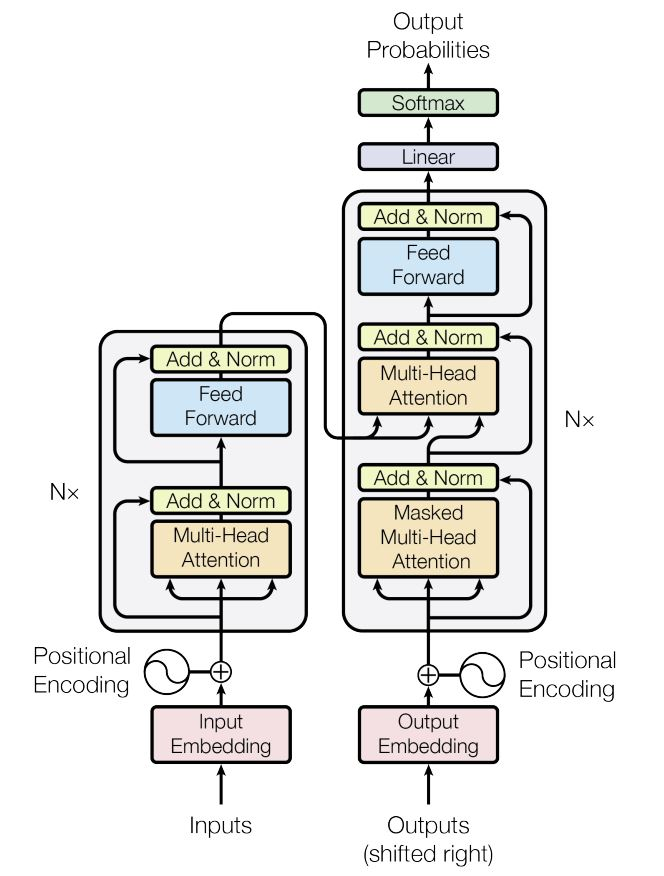
\includegraphics[width=0.5\textwidth]{chapters/images/Transformer/Architecture.JPG}
    \caption{Model Architecture\cite{vaswani2017attention}}
    \label{fig:Model_Architecture}
\end{figure}

\subsection{Overview of transformer model architecture}

The transformer architecture is made of encoder and decoder as shown left and right respectively in \Cref{fig:Model_Architecture}. A Comprehensive introduction of components and its functionality is described in paragraphs below.

\subsubsection{Input Embedding}
It is the first component in both encoder and decoder. This layer takes input sequence and convert it into vectors that is also known as continuous representation. It maps each word  and provide numerical value to each word.

\subsubsection{Positional encoding}
In this step, the positional information is being injected to the vector representation derived from input embedding layer. Transformer uses wave function to give positional information to input embedding by creating vectors for odd and even positions using cosine and sine function respectively (\Cref{eq:Wave_functions}).

\begin{equation}
    \label{eq:Wave_functions}
    PE_{(pos, 2i)} = \sin{\left(\frac{pos}{10000^\frac{2i}{d_{model}}}\right)}
\end{equation}
\[PE_{(pos, 2i+1)} = \cos{\left(\frac{pos}{10000^\frac{2i}{d_{model}}}\right)} \]

\subsubsection{Encoder Layer}


\begin{figure}[ht]
    \centering
    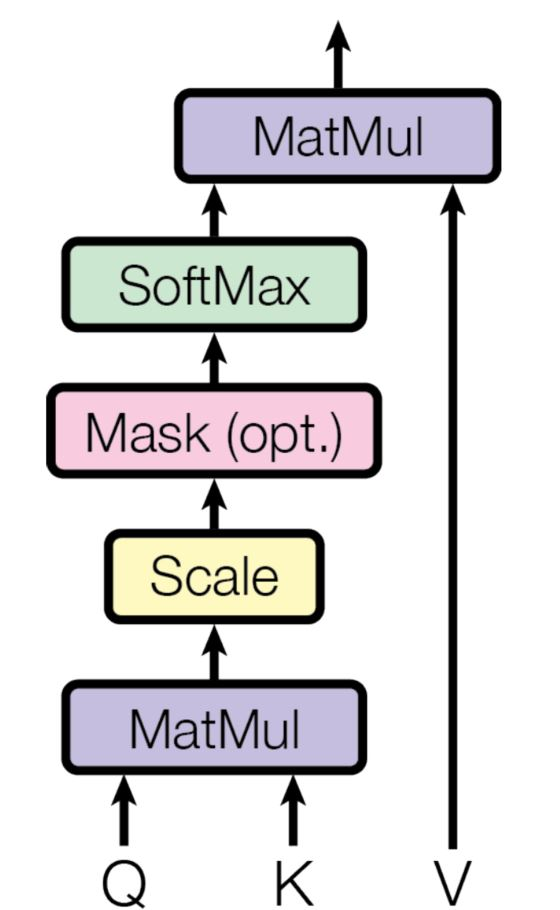
\includegraphics[width=0.25\textwidth]{chapters/images/Transformer/Inside_Attention.JPG}
    \caption{Scaled Dot-product Attention \cite{vaswani2017attention}}
    \label{fig:Scaled_Dot-product_Attention}
\end{figure}

The encoder layer is made of two sub-layer, multi-headed attention followed by fully connected feed forward network (\Cref{fig:Model_Architecture}). Multi-headed attention layer uses self-attention that allows the model to associate each word to other words in input embedding. To achieve self-attention, input embedding are passed through three linear layers to obtain query, key and value vectors represented as Q, K and V in \Cref{fig:Scaled_Dot-product_Attention}. As an example, if a word or sentence we used to search something in Google search are queries, the websites that Google search will provide are keys and the content of the websites are Values. Matrix multiplication step uses these queries and keys to obtain score matrix. The score matrix shows how much attention a word should keep into other words. These scores are then divided using square root of the dimension of queries and keys to scale it down to obtain stable gradients during values multiplication. After that the softmax is being taken to get the attention weights or attention filter. Softmax is a function that takes each vectors from scale matrix, normalizes it and gives the probabilistic distribution so that each component in matrix will be in interval of (0,1). By doing so, the higher score will be heightened and lower scores will be depressed providing model confident values to attend words accordingly. Later on, these attention weights are multiplied with value vectors (\Cref{eq:Attention}). The higher softmax scores will keep the word that is more important and lower softmax scores will soften the words that are irrelevant. After that query, key and value vectors are splited into N vectors and applied to self-attention individually therefore known as multi-headed attention computation where each self-attention process is called head. Each head will produce output vector which will be concatenated into a single vector. This way each head will learn something different than other layers. 
\begin{equation}
    Attention(Q,K,V) = softmax\left(\frac{QK^T}{\sqrt{d_k}}\right)V
    \label{eq:Attention}
\end{equation}


\begin{figure}[hb]
    \centering
    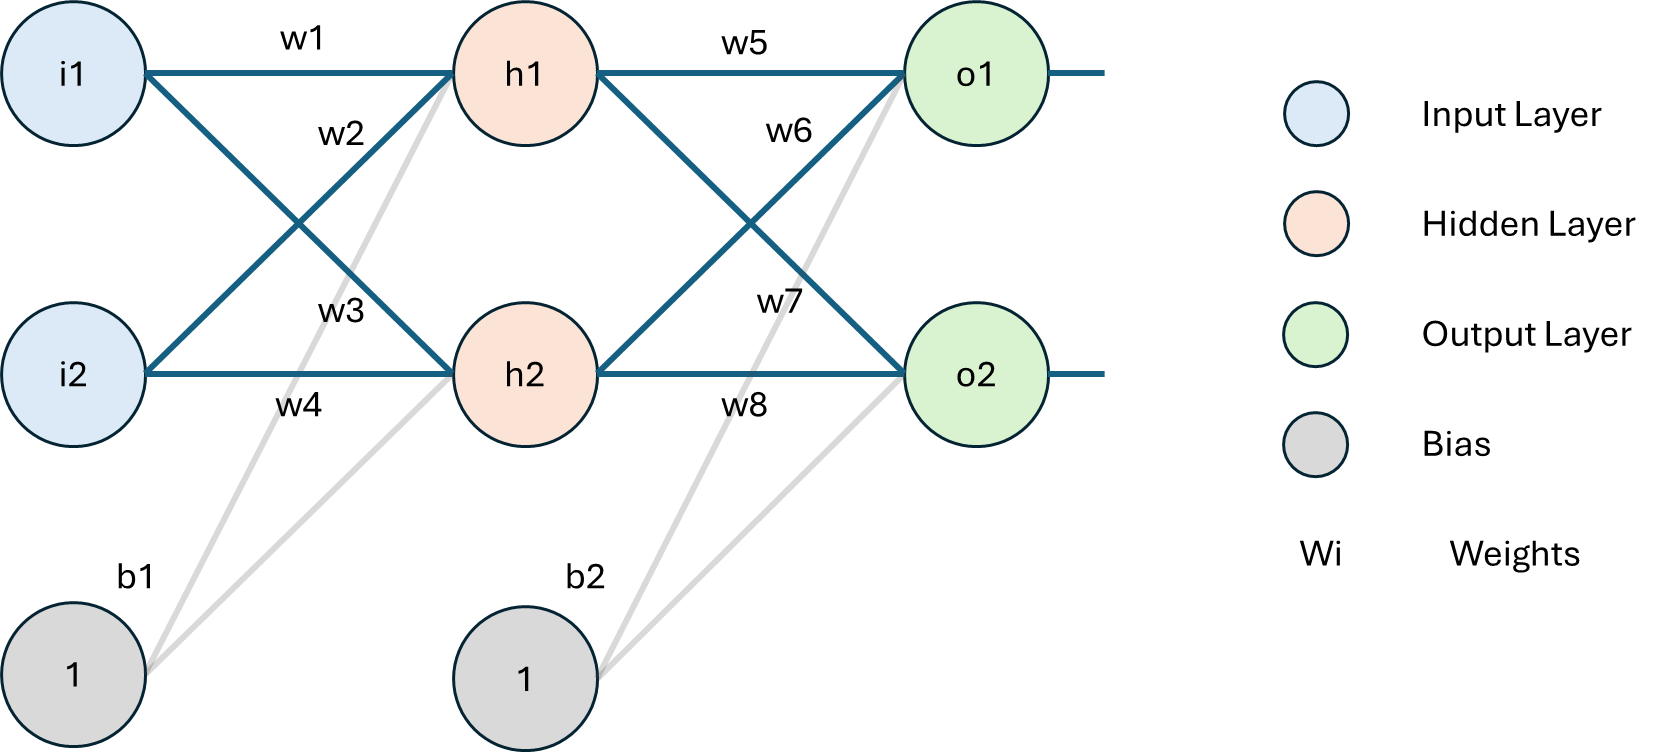
\includegraphics[width=0.7\textwidth]{chapters/images/Transformer/neuralnet.png}
    \caption{Diagram of neural network with different layers}
    \label{fig:neuralnet}
\end{figure}

The block "Feed Forward" in \Cref{fig:Model_Architecture} refers to the term multi-layered networks of neurons and information in these layers flows into one direction hence is pronounce feedforward. The network is made of Input Layer, Hidden Layer and Output Layer. In \Cref{fig:neuralnet} a simple neural network with two input, two hidden and output neurons has been shown. The goal is to find a weights for hidden layer and output layer in a way that Network takes the input and compute with these weights assigned to hidden and output neurons and try to predict the desired or nearest output. In initial phase, these weights assigned to hidden layer and output layer can be random or the attention derived from attention mechanism. In the process Forward Pass, the input values are passed to hidden layers. Total input value will be derived at each hidden node and then being squash using activation function like ReLU \cite{ReLU}, tanh \cite{tanh}. These activation functions help neural network to be non-linear allowing neural networks to expand complex representations and functions that is not possible with a linear regression model. Weights shows the strength of the connection between layers and biases make sure that if the input value is 0 than in activation function the output is not 0. The process is repeated for the output layer using the output of hidden layer as a inputs. Once we receive the outputs at output layers based on initial weights, the total error is being calculated based on targeted values. Once we have the total error of the network the process "Backwards pass" starts in which algorithm like "backpropagation" is used to calculate the gradient according to the total error using "Chain rule" for each node. Sometimes the learning rate is being used to multiply this gradient with the learning rate and then subtracted from the initial weights resulting in new weights. Then the process is repeating but this time with the new weights and is being repeated until the network provide outputs near to the targeted value. 

All these operation serves the prime purpose of encoding the input into a continuous representation with attentions so that decoder can focus on suitable word in the input while decoding. One can stack the encoder layers to encode the inputs in order to further encode the information. By doing so each layer can learn different attention representation that boosts the predictive power of the transformer network. 

\subsubsection{Decoder layer}
The decoder is responsible to generate the text sequences from the output vectors from encoder. It has similar sub layers as the encoder one multi-headed attention layers and feed-forward layer. The decoder is auto regressive that uses the previous outputs as inputs and uses encoder outputs that includes the attention information from input.

The input goes to embedding layers to obtain positional embedding. After that, these position aware vectors goes through multi-headed attention layer to generate the scores which later will be used as a decoder input. The next multi-headed attention layers works slightly different. Due to the fact that decoders are autoregressive and omit the sequence word-by-word, a condition is applied where it uses the positions to insure that prediction for position $i$ can only depend on known outputs at positions less than $i$. This process also known as mask where all the position greater than $i$ will be assigned as negative infinity so that when the softmax will be performed, there will be zero attention scores for future tokens. The output of the first multi-headed attention layer is mask output vector which will be used as a values for second multi-headed attention and the encoder output will be taken as keys and queries. The output second multi-hesded attention layer goes through to feed forward where the output will go through linear layer that act as a classifier, Here, the softmax layer will provide probaility score to each class between 1 and 0. The one with highest probability score will be taken as predicted word. The decoder can also be stacked N times that takes inputs from the encoder and the layers before it, which helps model to focus and extract on different combinations of attention, attention heads resulting in a boost in predictive power.
% \begin{equation}
%     Attention(Q,K,V) = softmax\left(\frac{QK^T}{\sqrt{d_k}}\right)V
%     \label{eq:Attention}
% \end{equation}





% Most used structure for transforming sequence is encoder-decoder. Where encoder uses input sequence as $(x_1, x_2, ..., x_n)$ and convert it into continuous representations (numerical representation) z = $(z_1, z_2, ..., z_n)$. The decoder takes this given z and generates an output sequence $(y_1, y_2, ..., y_n)$ using one element at a time. Model is auto-regressive at each steps \cite{graves2013generating}, that uses the former result as a additional input in order to generate the next result. The Transformer uses this overall architectures in addition with self-attention with connected encoder and decoder (left and right respectively in Figure \ref{fig:Model_Architecture}).






% The encoder contains 6 identical layers where each layers contains two sub-layers. The first layer is a multi-head self-attention mechanism and second layer is feed-forward network. Each sub-layers of this layers is using residual connections \cite{he2016deep} (please refer to \ref{residual_connection}) which will be normalized using normalization layer \cite{ba2016layer} resulting LayerNorm(x+Sublayer(x)). Sublayer(x) is the function implemented by sub-layer itself. All these residual connections, sub-layers and embedding layers produces outputs of 512 dimension. Decoder also contains 6 layers with its sub-layers. Decoder takes the output of Encoder layer and performs self-attention, uses residual connections with normalization. In Decoder, the self-attention sub-layer is modified where it uses the positions to insure that prediction for position $i$ can only depend on known outputs at positions less than $i$.

% \subsection{residual connections \label{residual_connection}}
% \cite{Residual_connection}




% \subsection{Attention Mechanism\label{attention}}
% Transformer became prime component in natural language processing due to its ability to process long text and generate results and text while maintaining the context. Figure \ref{fig:Scaled_Dot-product_Attention} shows different components of "Multi-Head Attention" layer in Figure \ref{fig:Model_Architecture}. Where Q, K and V represents Query, Key and Value respectively. As an example, Query can be a word or sentence we used to search something in google search, Keys can be the websites that google search will provide which is similar to query and Value can be the content of the websites. The similarity between Query and Key are computed using \textbf{Cosine Similarity} ranging from +1 to -1. In Figure \ref{fig:Model_Architecture} in both encoder and decoder, Inputs are simply embedding of words, a fixed-length vectors. Machine translation algorithm like RNN, CNN and LSTM takes one input embedding at a time in a sequential manner, while Transformers take all embedding as a whole, Hence the \textbf{Positional Encoding} has been introduced in order to add information of word order to the vectors. In paper \cite{vaswani2017attention}, positional encoding has been achieved using wave frequencies \ref{eq:Wave_functions} to provide each word a unique position embedding.





% Once we have position aware matrices of Query, Key and Value, the steps mentioned in Figure \ref{fig:Scaled_Dot-product_Attention} will be performed in which in the step "MatMul" the dot product of matrices Q and K is being taken in order to find similarity also known as providing score. In step "Scale" we divide the score in order to scale, \(\sqrt{d_k}\) is used in paper \cite{vaswani2017attention} where \(d_k\) represents dimension of keys. In the next step the Softmax is being taken in order to squash the results between 0 and 1 at this stage the resultant matrix is so called \textbf{Attention Filter}. Finally, multiplying this Attention Filter to Value matrix gives us the \textbf{Attention} \ref{eq:Attention}.

% \begin{equation}
%     Attention(Q,K,V) = softmax\left(\frac{QK^T}{\sqrt{d_k}}\right)V
%     \label{eq:Attention}
% \end{equation}

% \subsection{Feed Forward\label{feed forward}}
% \begin{figure}[ht]
%     \centering
%     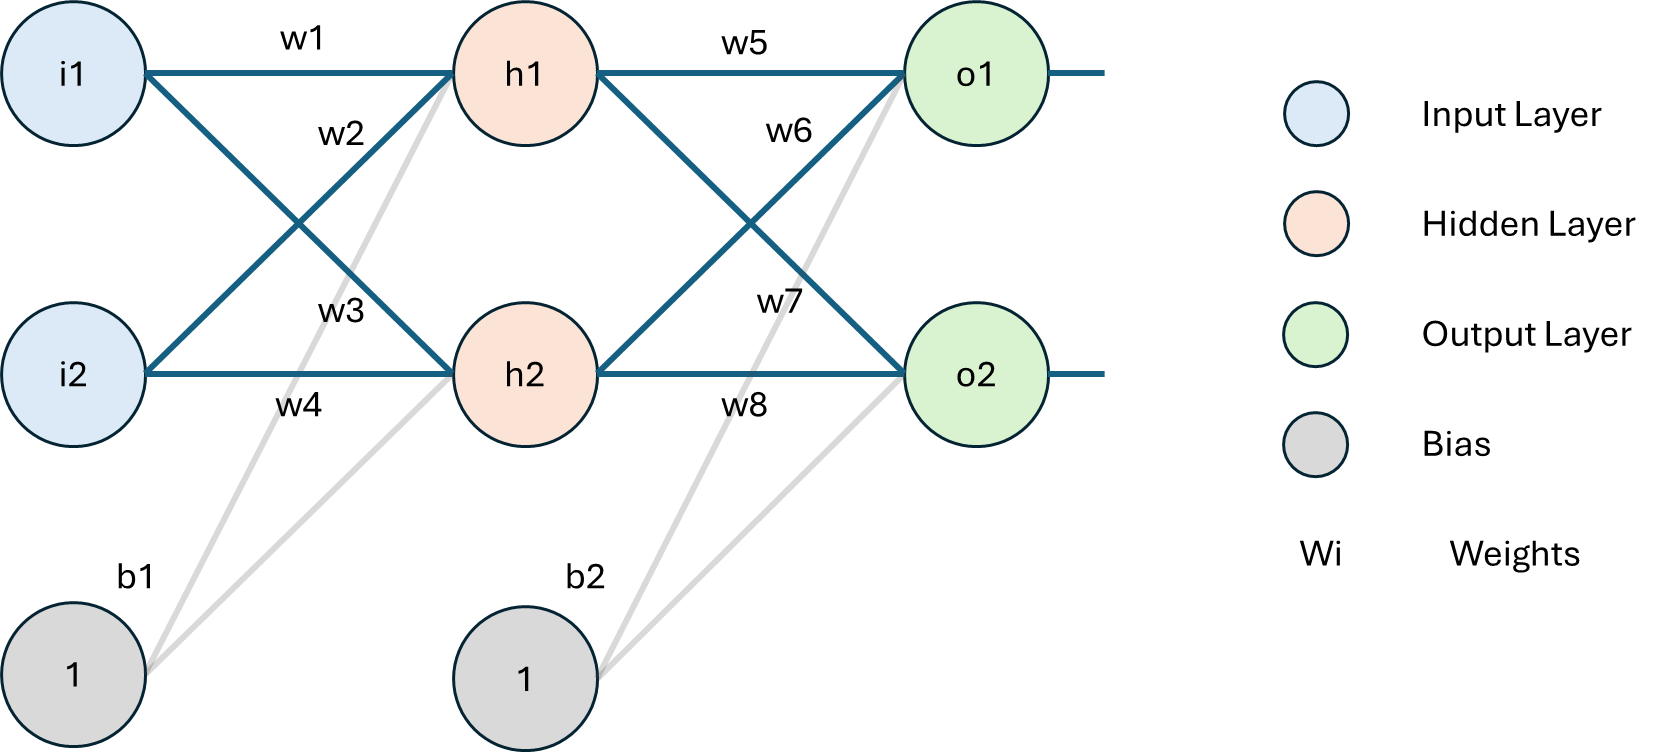
\includegraphics[width=0.7\textwidth]{chapters/images/Transformer/neuralnet.png}
%     \caption{Diagram of neural network with different layers}
%     \label{fig:neuralnet}
% \end{figure}

% The block "Feed Forward" in figure \ref{fig:Model_Architecture} refers to the term multi-layered networks of neurons and information in these layers flows into one direction hence is pronounce "feedforward". The network is made of Input Layer, Hidden Layer and Output Layer. In Figure \ref{fig:neuralnet} a simple neural network with two input, two hidden and output neurons has been shown. The goal is to find a weights for hidden layer and output layer in a way that Network takes the input and compute with these weights assigned to hidden and output neurons and try to predict the desired or nearest output. In initial phase, these weights assigned to hidden layer and output layer can be random or the attention derived from attention mechanism. In the process Forward Pass, the input values are passed to hidden layers. Total input value will be derived at each hidden node and then being squash using activation function like ReLU \cite{ReLU}, tanh \cite{tanh}, Softmax and so on. These activation functions help neural network to be non-linear. Weights shows the strength of the connection between layers and biases make sure that if the input value is 0 than in activation function the output is not 0. The process is repeated for the output layer using the output of hidden layer as a inputs. Once we receive the outputs at output layers based on initial weights, the Total Error is being calculated based on targeted values. Once we have the total error of the network the process "Backwards pass" starts in which algorithm like "backpropagation" is used to calculate the gradient according to the total error using "Chain rule" for each node. Sometimes the learning rate is being used to multiply this gradient with the learning rate and then subtracted from the initial weights resulting in new weights. Then the process is repeating but this time with the new weights and is being repeated until the network provide outputs near to targeted value. 


\section{Pre-Training And Fine-Tunning}

The concept of pre-training comes from transfer learning \cite{Transfer_learning} and the core idea is to reuse previously learned knowledge from one or more task and apply it to a new task. The majority of deep learning methods are dependent on high quality labeled data. Labeling data manually can be expensive and time consuming. Pre-training methods allows models to use unlabeled data such as books, articles, websites and so on and helps models to identify patterns, structures and semantic knowledge that is present in the corpus. pre-training generally refers to train the models on these large amount of unlabeled corpus to enhance the initial parameters of the neural networks and fine-tune refers to further training these models on specific targeted task using supervised learning to improve performance in that sepcific tasks. The prime advantage of these methods was the ability to deal with more than one task for instance question answering, text classification, language generation and so on. In generative pre-training (GPT) \cite{radford2018improving} such approach has been discussed for language understanding task using transformer architecture and combination of unsupervised pre-training and supervised fine-tuning.

Pre-training has enabled a breakthrough in the domain of NLP. Prior to pre-trained model(PTM) there was a requirement of designing a models according to target specific tasks and these trained model can not be used other than that particular tasks. The emergenece of PTMs made it possible to serve models as a foundational model which started a new paradigm for NLP. For instance BERT, a pre-trained model from Google took 16 TPU (Tensor Processing Units) chips for \(BERT_{BASE}\) and 64 TPU chips for \(BERT_{LARGE}\) and 4 days for each model to complete the training \cite{devlin2018bert}. BERT is open-source and one can simply use it for downstream task with fine-tune in desired tasks and save amount of computation power and time it took to train this model.
%In addition, models like \cite{T5} is able to perform two tasks such as language understanding and generation task. 

\section{Cloud Computing}

Internet keeps changing the way people work, learn, communicate and so on. It has influenced from one individual to entire industries. Rapid development of processing and storage technologies helped to reduce the cost of computing while increasing power and availability. This technological advancement provided a realization of a computing model called "Cloud Computing". Users can lease and release the resources like CPU and Storage in an on-demand manner. In general, the cloud computing infrastructure can be divided into two prime roles. One, the infrastructure provider responsible to manage cloud platforms. Second, service-provider, who consume these resources from infrastructure-providers and servers different services to end users. Cloud technologies have influenced the Information Technology (IT) industries and Companies like Google, Microsoft and Amazon provides cloud-platforms which help enterprises to develop, reshape their business models and gain benefits such as No up-front investment in resources since now they can just rent the infrastructure as they uses also known pay-as-you-go pricing model, High scalability, Easy access and important one Risks and maintenance. Using cloud infrastructure means we are simply outsourcing the risks such as hardware failures to the infrastructure providers who are better equipped to manage these risks and decreasing the cost on maintenance and training of staff. In paper \cite{lee2013view}, Author presents results of an economic view of IBM cloud computing engagements \ref{tab:IT_benifits}.


\begin{table}[hb]
    \centering
    \begin{tabular}{|c|c|c|c|}
    \hline
         & Tasks & Traditional Computing &  Cloud Computing \\
    \hline
    \multirow{6}{5em}{Increasing speed and flexibility} & Test provisioning & Weeks & Minutes \\ 
        & Change Management & Months & Days/hours \\ 
        & Release Management & Weeks & Minutes \\
        & Service Access & Administered & Self-service \\ 
        & Standardization & Complex & Reuse/Share \\
        & Metering/billing & Fixed Cost & Variable Cost \\
    \hline
    \multirow{2}{5em}{Reducing Costs} & Server/storage utilization & 10-20\% & 70-90\% \\
        & Payback period & Years & Months \\
    \hline
    \end{tabular}
    \caption{Benifits of Cloud Computing}
    \label{tab:IT_benifits}
\end{table}



\subsection{Overview of cloud Architecture}

The architecture of cloud computing environment is made of sublayers such as Infrastructure as a service (Iaas),  Platform as a Service (Paas) and Software as a Service (SaaS) as show in \Cref{fig:Layers_of_Cloud_Architecture}. Each layer is coupled with layers above or below in a way that each layer can evolved separately allowing applications to be better at management and maintenance. 

\begin{figure}[ht]
    \centering
    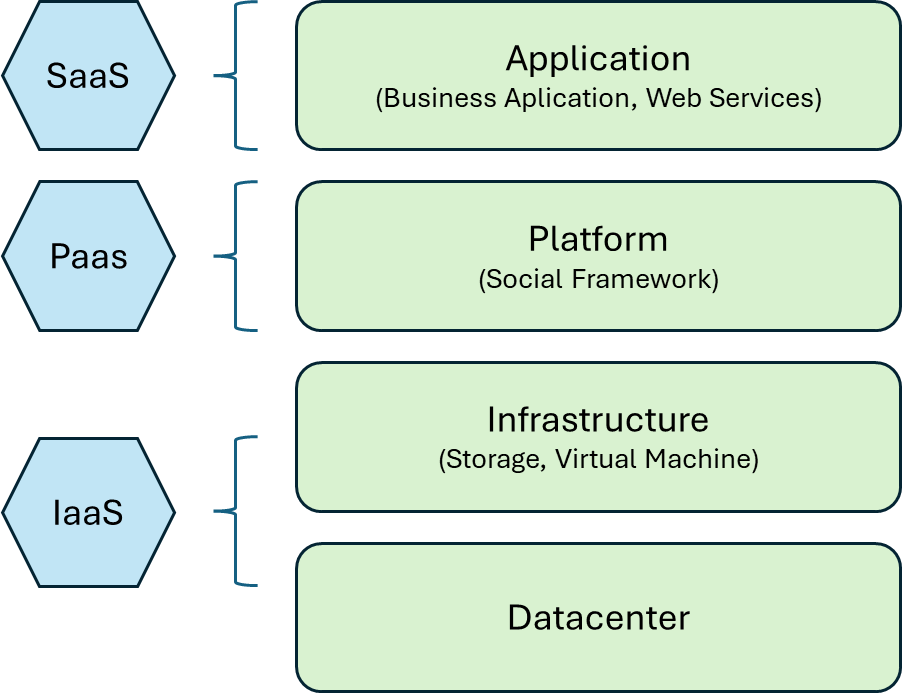
\includegraphics[width=0.5\textwidth]{chapters/images/Cloud_Computing/Cloud_layers.png}
    \caption{Layers of Cloud Architecture}
    \label{fig:Layers_of_Cloud_Architecture}
\end{figure}

\subsubsection{Infrastructure as a Service - IaaS}
The layer IaaS includes resources like data centers that contains servers, routers, power and cooling systems and so on. Therefore, also known as a hardware layer. It also contains the infrastructure layer that includes pool of storage and computing resources like virtualization technologies therefore also known as virtualization layer. IaaS usually refers to providing resources on-demand mostly in forms of Virtual Machines for instance Amazon EC2 \cite{AWS_ec2}. 

\subsubsection{Platform as a Service - PaaS}

This layer is build on top of the infrastructure layer that includes different operating systems and application frameworks. PaaS-provider delivers necessary hardware and software tools over internet for users which allows to focus on deployment and management of their application. 

\subsubsection{Software as a Service - SaaS}

Saas is the layer where the actual cloud application is being served that reaches to end-user and it is at the top of the hierarchy. It is different from ordinary served application in terms of highly-scalable since this layers have automatic-scaling feature to achieve better performance, availability and lower operating cost.

\subsubsection{Machine Learning and Cloud Computing}

Cloud infrastructure outperforms the traditional way of serving the ML models in terms of performance and cost, many of these cloud provider are focusing on developing new architectures that are specifically developed for workloads like neural networks and deep learning, Implementing features like specialized cores to increase matrix operations for instance Google TPUs (Tensor Processing Units) \cite{google_tpu}. In addition, the elasticity, flexibility and economy is making cloud computing more suitable for deploying machine learning models. The different layer model of cloud makes it easy to deploy various infrastructure components on different layers that helps to manage these resources in efficient ways. Cloud providers offers inbuilt PaaS and SaaS a step ahead from low-level offerings like IaaS to enable large-scale computing infrastructures with easy-to-use services in respect to Machine learning "as-a-Service" for end users. Today's data-centers are located in various part of the world. Using services available in PaaS/ SaaS one can deploy their services or product on distributed infrastructures which is accessible trough internet. 

Cloud computing enabled companies to build their products and collaborate on a global level. For instance Hugging face \cite{huggingfacehub} provides a platform where companies or individuals can build their own AI, leverage open source models and technology and make it easy for data scientist, machine learning engineers and developers to collaborate. Users can easily access these models and applications with the hardware capabilities of Google Cloud \cite{Googlecloud} such as TPU instances, Virtual Machines, NVIDIA H100 Tensor Core GPUs \cite{Nvidiagpu} and so on. Currently, there are approx more than 400 thousand models, 150 thousand application and 100 thousand datasets available on hugging face \cite{huggingfacehub}. Some of them may come with copyrights or Licences to use and assets like  Open-Source, anyone can access to these pre-trained models which are already well trained and architected, one can fine-tune it and use it for their downstream tasks with their own datasets or the available datasets without investing on large resource required to set up IT infrastructure to serve high computing services like machine learning on Hugging face by just using internet through their laptops in a pay-as-you-go manner.






